\documentclass[../../../interview-questions.tex]{subfiles}

\begin{document}

\subsection{Java类文件结构}

Java类文件结构如下表\footnote{参考:\url{https://en.wikipedia.org/wiki/Java_class_file}}所示:

\begin{table}[htbp]
	\caption{Java类文件结构}
	\label{table:mapo2}
	\begin{center}
		\begin{tabular}{cp{5cm}c}
			\hline
			\multirow{1}{*}{占用大小}
			& \multicolumn{1}{c}{字段描述} 
			& \multicolumn{1}{c}{数量}\\			
			\cline{1-3}
			4bit &  magic:魔数,用于标识文件类型,对于java来说是0xCAFEBABE  &  1 \\
			\hline
			2bit &  minor\_version:次版本号 & 1 \\
			\hline
			2bit &  major\_version:主版本号 & 1 \\
			\hline							
		\end{tabular}	
	\end{center}
\end{table}

使用javap输出常量表:

\begin{figure}[htbp]
	\centering
	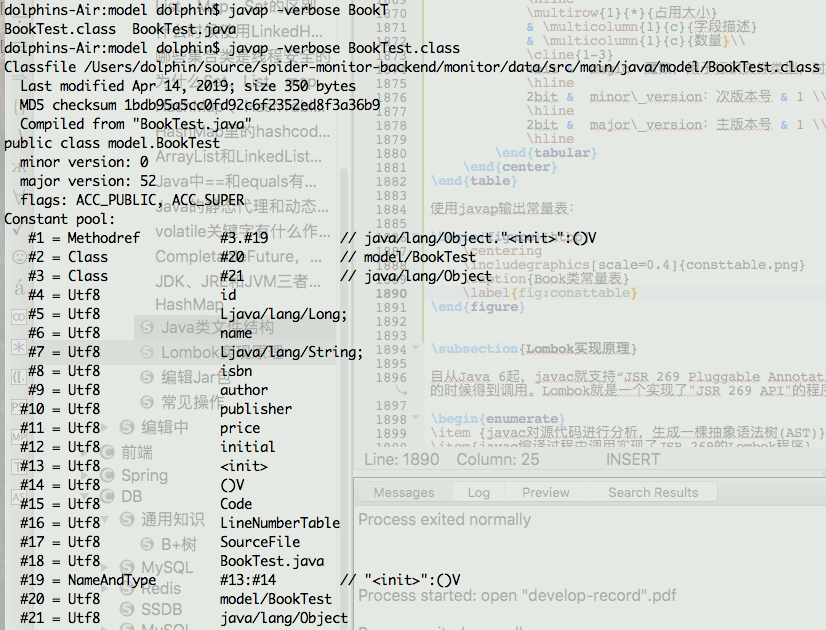
\includegraphics[scale=0.5]{consttable.png}
	\caption{Book类常量表}
	\label{fig:consttable}
\end{figure}

\end{document}